\chapter{Lecture 7: More on Power Series}

\begin{theorem}
    [Differentiation of Power Series]
    Consider a power series
    $$ \sum_{n=0}^{\infty} a_n (z-z_0)^n \qquad \text{with } 0 < R \leq \infty $$
    Then: $f(z) = \sum_{n=0}^{\infty} a_n (z-z_0)^n$ is \textbf{\textit{analytic}} in the disc $\{|z-z_0| < R\}$ and
    $$\frac{d }{dz} f(z)= \sum_{n=1}^{\infty} n a_n (z-z_0)^{n-1} $$
\end{theorem}

\begin{example}
    [Proof of Convergence of Power Series Differentiation]
    Show that
    $$\frac{d }{dz} f(z)= \sum_{n=1}^{\infty} n a_n (z-z_0)^{n-1} $$
    converges for $|z-z_0| < R$.

    \begin{proof}
        Let $|z-z_0| < R$. and let $r < s < R$. then, $\exists N | \forall n \geq N$ we have.
        $$nr^{n -1} \leq S^n$$
        Since $\frac{r}{s} < 1$, by the ratio test:
        $$\lim_{n \to \infty} n(\frac{r}{s})^{n-1} = 0$$
        Thus:
        \begin{align*}
            \sum_{n  = 1}^{\infty} n|a_n|r^{n - 1} & \leq \sum_{n = 1}^{N} n|a_n|r^{n - 1} + \sum_{n = N}^{\infty} n|a_n|s^{n} \\
                                                   & \leq \sum_{n = 1}^{N} n|a_n|r^{n - 1} + \sum_{n = 1}^{\infty} n|a_n|s^{n} \\
        \end{align*}
        Of course $\sum_{n = 1}^{\infty} |a_n|s^{n}$ converges by the ratio test since $s < R$. Hence $\sum_{n = 1}^{\infty} n|a_n|r^{n - 1}$ converges.
    \end{proof}
\end{example}

\begin{theorem}
    [Infinite Differentiation of Power Series]
    if $f(z) = \sum_{n=0}^{\infty} a_n (z-z_0)^n$ has radius of convergence $0 < R \leq \infty$, then in the disc $\{|z-z_0| < R\}$, $f(z)$ is infinitely differentiable and
    $$f^{(m)}(z) = \sum_{n=m}^{\infty} n(n-1)\ldots(n-(m-1)) a_n (z-z_0)^{n-m} \qquad k = 1, 2, \ldots $$
\end{theorem}

\section{Cauchy's Theorem}

\begin{definition}
    A domain $D$ is \textit{simply-connected} if, whenever $\gamma$ is a closed curve in $D$, the inside of $\gamma$ is also a subset of $D$. \\
    \textit{Informally}, a domain is simply connected if it has no holes.
\end{definition}

\begin{figure}[H]
    \centering
    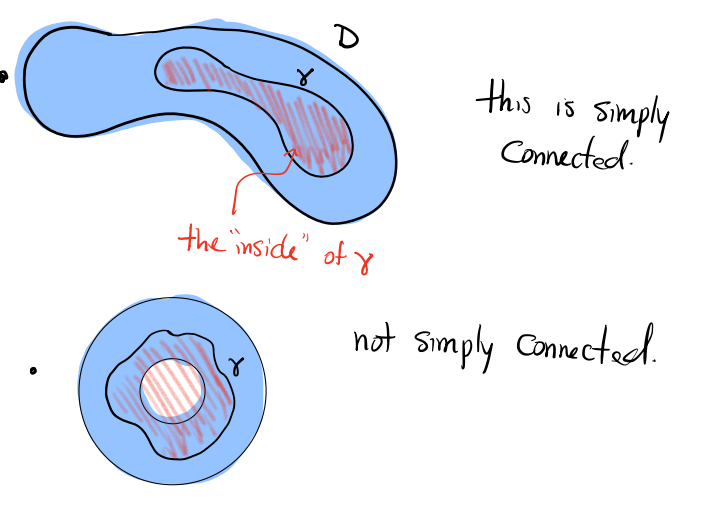
\includegraphics[width=0.5\textwidth]{LECTURE_7/simply-connected.png}
    \caption{Simply Connected Domain}
\end{figure}

\begin{theorem}
    [Cauchy's Theorem]
    Suppose $f$ is analytic on a domain $D$, and let $\gamma$ be a $C^1$ simple closed curve in $D$ such that the inside of $\gamma = \Omega \subset D$. Then:
    $$\oint_{\gamma} f(z) dz = 0$$
\end{theorem}

\begin{proof}
    By Green's Theorem:
    $$\oint_{\gamma} f(z) dz = i\iint_{\Omega} \left(\frac{\partial f}{\partial x} - \frac{\partial f}{\partial y}\right) dxdy$$
    But if $f = u + iv$ is analytic, so:
    \begin{align*}
        \frac{\partial f}{\partial x} & = \frac{\partial u}{\partial x} + i \frac{\partial v}{\partial x}                 \\
                                      & = \frac{\partial v}{\partial y} - i \frac{\partial u}{\partial y}                 \\
                                      & = -i \left(\frac{\partial u}{\partial y} + i \frac{\partial v}{\partial y}\right) \\
                                      & = -i \frac{\partial f}{\partial y}
    \end{align*}
    So $\frac{\partial f}{\partial x} + i \frac{\partial f}{\partial y} = 0$ and the result follows.
\end{proof}

\begin{theorem}
    [More General Cauchy's Theorem]
    if $D$ is a simply connected domain and $\gamma$ is any closed, piecewise $C^1$ curve in $D$, then, if $f$ is analytic on $D$:
    $$\oint_{\gamma} f(z) dz = 0$$
    \begin{figure}[H]
        \centering
        \begin{subfigure}{0.5\textwidth}
            \centering
            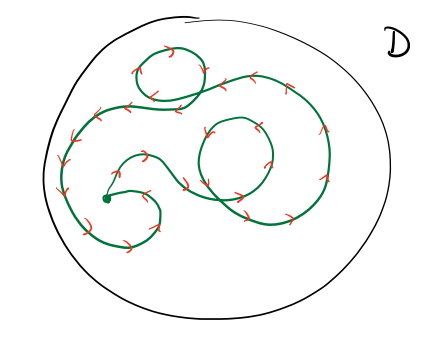
\includegraphics[width=0.5\textwidth]{LECTURE_7/1.png}
            \caption{Simply Connected Domain in $D$}
        \end{subfigure}
        \begin{subfigure}{0.5\textwidth}
            \centering
            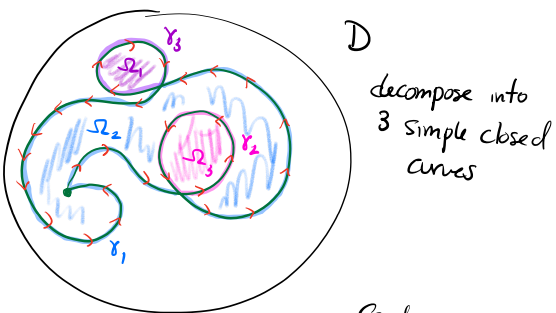
\includegraphics[width=0.5\textwidth]{LECTURE_7/2.png}
            \caption{Decomposition of $\gamma$}
        \end{subfigure}
    \end{figure}
    $$ \oint_{\gamma} f(z) dz = \oint_{\gamma_1} f(z) dz + \oint_{\gamma_2} f(z) dz +  \oint_{\gamma_3} f(z) dz = 0$$
\end{theorem}

\begin{theorem}
    [Differentiability of Analytic Functions]
    If $D$ is a simply connected domain and f is analytic on $D$, then there is an analytic function $F$ on $D$ such that $F^\prime = f$.
\end{theorem}
\begin{lemma}
    For $F(z) = \int_{\gamma}f(z)dz$, $F$ is independent of the path $\gamma$.
\end{lemma}
\begin{proof}
    Let's say $\gamma_1$ and $\gamma_2$ are two paths from $z_0$ to $z_1$, and $\Gamma = \gamma_1 - \gamma_2$. Then:
    \begin{align*}
        \oint_{\Gamma} f(z) dz & = \oint_{\gamma_1} f(z) dz - \oint_{\gamma_2} f(z) dz \\
        0                      & = F_1 - F_2                                           \\
        F_1                    & = F_2
    \end{align*}
    \begin{figure}[H]
        \centering
        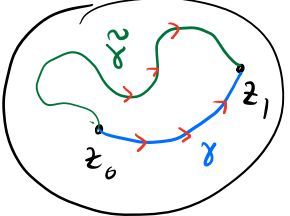
\includegraphics[width=0.5\textwidth]{LECTURE_7/independent.png}
    \end{figure}
\end{proof}
\begin{theorem}
    [Cauchy's Integral Formula]
    Suppose $f$ is analytic on a domain $D$, $\gamma$ is piecewise $C^1$, positively oriented, simple closed curve in $D$ such that: $\text{inside}( \gamma) = \Omega \subset D$. Then:
    $$f(z_0) = \frac{1}{2\pi i} \oint_{\gamma} \frac{f(\xi)}{\xi - z} d\xi\qquad \forall z \in \Omega$$
\end{theorem}

\begin{proof}
    \begin{figure}[H]
        \centering
        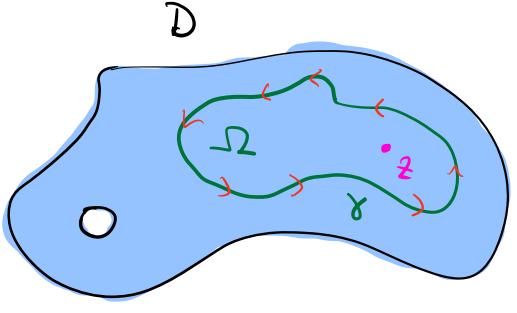
\includegraphics[width=0.5\textwidth]{LECTURE_7/cauchy-integral.png}
    \end{figure}
    Let $g(\xi) = \frac{f(\xi)}{\xi - z}$ be an analytic function in $\Omega/\{z\}$.\\
    Let $D_{\epsilon}(z) = \{z \in \mathbb{C} | |z - z_0| < \epsilon\}$ be a disc of radius $\epsilon$ centered at $z_0$.\\
    We choose $\epsilon$ to be small such that $D_{\epsilon}(z) \subset \Omega$.\\
    By Cauchy's Theorem:
    \begin{align*}
        \oint_{\gamma} \frac{f(\xi)}{\xi - z} d\xi & = \oint_{\partial D_{\epsilon}(z)} \frac{f(\xi)}{\xi - z} d\xi
    \end{align*}
    \textit{Note: $\partial D_{\epsilon}(z)$ is the boundary of $D_{\epsilon}(z)$}.\\
    Now we parametrize $\partial D_{\epsilon}(z)$ by $\partial D_{\epsilon} = z + \epsilon e^{i\theta}$, $0 \leq \theta \leq 2\pi$, Then:
    \begin{align*}
        \oint_{\partial D_{\epsilon}(z)} \frac{f(\xi)}{\xi - z} d\xi & = \int_{0}^{2\pi} \frac{f(z + \epsilon e^{i\theta})}{\epsilon e^{i\theta}} \epsilon i e^{i\theta} d\theta \\
                                                                     & = i \int_{0}^{2\pi} f(z + \epsilon e^{i\theta}) d\theta
    \end{align*}
    as $\epsilon \to 0$, $f(z + \epsilon e^{i\theta}) \to f(z)$ (by continuity of $f$).\\
    Hence:
    \begin{align*}
        \lim_{\epsilon \to 0} i \int_{0}^{2\pi} f(z + \epsilon e^{i\theta}) d\theta & = 2\pi i f(z) \\
    \end{align*}
    Thus
    $$\boxed{\oint_{\gamma} \frac{f(\xi)}{\xi - z} d\xi = 2\pi i f(z)}$$
\end{proof}

\section{Applications of Cauchy's Integral Formula}

\begin{example}
    Compute:
    $$\int_{0}^{2\pi} \frac{d\theta}{2 + \sin \theta}$$

    \hrule
    \vspace{1em}
    \textbf{\underline{Idea:}} Write this as an integral for an analytic function over the circle $z = e^{i\theta} \quad 0 \leq \theta \leq 2\pi$. \\
    If $|z| = 1$, then
    \begin{align*}
        \sin \theta        & = \frac{e^{i\theta} - e^{-i\theta}}{2i} \\
                           & = \frac{z - z^{-1}}{2i}                 \\ \\
        \therefore d\theta & = \frac{dz}{iz}
    \end{align*}
    So, integral is:
    \begin{align*}
        \int_{\gamma(\theta) = e^{i\theta}} \frac{1}{2 + \frac{z - z^{-1}}{2i}} \frac{dz}{iz} & = \int_{\gamma} \frac{2dz}{4iz + (z^2 - 1)}                                                                                \\
        \rightarrow z^2 - 4iz - 1                                                             & = \left[z - \left(\frac{-4i + \sqrt{-16 + 4}}{2}\right)\right]\left[z - \left(\frac{-4i - \sqrt{-16 + 4}}{2}\right)\right] \\
                                                                                              & = (z - i(\sqrt{3}-2))(z + (\sqrt{3} + 2)i)
    \end{align*}
    Since $|\sqrt{3} - 2| < 1, |\sqrt{3} + 2| > 1$, we can apply the cauchy integral formula:
    \begin{figure}[H]
        \centering
        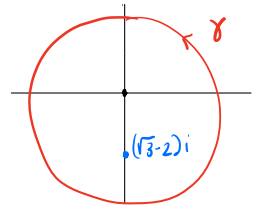
\includegraphics[width=0.5\textwidth]{LECTURE_7/example.png}
        \caption{Circle of Radius 1}
    \end{figure}
    \begin{align*}
        \int_{\gamma} \frac{1}{(z - i(\sqrt{3} - 2))}\cdot \frac{2dz}{(z + i(\sqrt{3} + 2))} & = 2\pi i \left(\frac{2}{(\sqrt(3)-2)i + (\sqrt{3} + 2)i}\right) \\
                                                                                             & = \frac{4\pi}{2\sqrt{3}}                                        \\
                                                                                             & = \frac{2\pi}{\sqrt{3}}
    \end{align*}
\end{example}